% !TEX root = ../TSG_Administrator's_Guide_SV20.11_v1.0_EN.tex
%
\pdfbookmark[0]{Objects}{Objects}
\chapter*{\hypertarget{link:Objects}{Objects}}
\label{sec:objects}

A policy object consists of one item or a set of collective items that groups discrete identities such as IP addresses, URLs, applications, or accounts. 
One policy object is allowed to reference same type objects as subordinate objects. Typically, when creating a policy object, you group objects that require similar permissions in policy. 
For example, you can group the set of server IP addresses as an address group policy object and reference the address group in the security policy. By grouping objects, 
you can significantly reduce the administrative overhead in creating policies. An object group is also considered as an object when referenced. 
You can reference the object group in policy instead of manually selecting multiple objects one at a time.

{
\color{linkblue}
\hyperlink{link:Objects Type}{> Objects Type} \\
\hyperlink{link:IP Addresses}{> IP Addresses} \\
\hyperlink{link:Subscriber IDs}{> Subscriber IDs}\\
\hyperlink{link:Categories}{> Categories}\\
\hyperlink{link:Applications}{> Applications}\\
\hyperlink{link:Configure Object Group}{> Configure Object Group}\\
}
\clearpage

You can create an object or create an object group. A policy object consists of one or multiple items, while an object group is composed of one or multiple subordinate objects. One object is allowed to reference same type objects as subordinate objects. 


To view object usages, please click column \textbf{Reference Count} of object list.


Then you will see\\
• Various policies for referencing the object; \\
• The group object that references the object.


Click the Graph button, you will see an object relationship graph. Policies, Proxy TCP Options, and parent objects that reference current object are displayed in the graph. 
As well as application signatures, which reference IP Address object when creating signatures with ip.src and ip.dst as Traffic Attribute. 
For more details, see \textbf{Advanced Setting} > \textbf{\hyperlink{link:Proxy TCP Option}{\color{linkblue}{Proxy TCP Option}}} and \textbf{Objects} > \textbf{Applications} > \textbf{\hyperlink{link:Signatures}{\color{linkblue}{Signatures}}}. 


Click the solid circle to unfold the referenced ancient object and click the hollow circle to fold the picture.


\notemark\textit{Note that direct or indirect self-reference is prohibited, i.e. A->A or A->B->A. Within the TSG system, object references can have up to six levels (from root node to leaf node).}


You can reference objects and object groups in your policies. Thus, you reduce the administrative overhead in creating policies. You can identify an object by its name or ID number. The object ID never changes even if you modify the object, such as when you change the object name. 


\pdfbookmark[1]{Objects Type}{Objects Type}
\section*{\hypertarget{link:Objects Type}{Objects Type}}
\label{sec:objects:type}

You can create the following policy objects on TSG. A policy object consists of one or multiple items, while an object group is composed of one or multiple subordinate objects.


\begin{longtable}{p{0.21\textwidth}|p{0.74\textwidth}}   
    \rowcolor{black}\multicolumn{1}{l!{\vlinewhite}}{\textcolor{white}{Policy Object}}  & \textcolor{white}{Description} \\\hline                                                                                                                                                          
    \tabincell{l}{IP Addresses/\\ Address Group} & IP Address contains three sub-types: IP, geography and IP Learning. The IP object can include an IPv4 or IPv6 address (single IP, range). Address Group Allow you to group specific source or destination addresses that require the same policy enforcement. You can then group a collection of address objects of the same type to create an address object group. IP learning type is not allowed to create group.\\ \hline                                                                                                                                                                                                            
    \tabincell{l}{FQDNs/\\FQDN Group} & That is fully qualified domain name to identify traffic. Using an FQDN object or FQDN object group reduces issues in environments where the host is subject to dynamic IP address changes. Support exactly matching and suffix matching.\\\hline 
    \tabincell{l}{Subscriber IDs/\\Subscriber ID\\ Group} & Allow you to create a list of Subscriber ID for RADIUS traffic. Support exactly matching only. \\\hline 
    \tabincell{l}{HTTP Signatures/\\HTTP Signature\\ Group} & Allow you to add keyword in Request as User-Agent and Cookie, in Response as Set-Cookie and Content-Type. Support exactly matching, prefix matching, suffix matching and substring matching. \\\hline 
    \tabincell{l}{Keywords/\\Keyword Group} &  A string you define that can be added as a filter in policy. You can enable Hex Mode. Support exactly matching, prefix matching, suffix matching and substring matching.
    

    \notemark\textit{Support maximum 8 substrings for AND expression. And when adding keyword for other objects, the same rule applies.}\\\hline 
    \tabincell{l}{URLs/\\URL Group} &  A Uniform Resource Locator, colloquially termed a web address, is a reference to a web resource that specifies its location on a computer network and a mechanism for retrieving it. A typical URL could have the form http://www.example.com/index.html, which indicates a protocol (http), a hostname (www.example.com), and a file name (index.html). Here the protocol is not allowed when adding. Support exactly matching, prefix matching, suffix matching, and substring matching \\\hline 
    \tabincell{l}{Categories/\\Category Group} &  Category classifies websites based on site content, features, and safety. Once created, the category can be selected as a filter of a policy. This means that a policy will only allow or block requests that match the category. For details, please refer to \hyperlink{link:Categories}{\color{linkblue}{Categories}}.\\\hline 
    \tabincell{l}{Accounts/\\Account Group} &  Stores the account information for your application. For example, you can add your email account as a filter when creating a policy using MAIL application. Support exactly matching, prefix matching, suffix matching and substring matching. \\\hline 
    \tabincell{l}{Applications} &  Applications, a patented traffic classification system available in TSG firewalls, determines what an application is irrespective of port, protocol, encryption or any other evasive tactic used by the application. It applies multiple classification mechanisms—application signatures, application protocol decoding, and heuristics—to your network traffic stream to accurately identify applications. An Application allows you to filter applications dynamically. \\\hline 
\end{longtable}


\notemark\textit{Description of matching method:}


\textit{• Substring matching, which has no wildcard character. E.g. “abc” is a substring of “abcde”.}


\textit{• Prefix matching, which is end with an asterisk character “*”. E.g. “abc*” is a prefix of “abcde”.}


\textit{• Suffix matching, which is begin with an asterisk character “*”. E.g. “*cde” is a suffix of “abcde”.}


\textit{• Exactly matching, which is begin with a dollar character “\$”. E.g. “\$abcde” is exactly same as “abcde”.}


\textit{• AND expression, which contains maximum 4 substrings. E.g. “abc” \& “cde” matches “abcde”.}


\textit{You could input nonprintable keyword in Hex mode. A valid hexadecimal keyword only contains “0~9” and “a~f”, and has even character number, e.g. “1a2b3c4d”.}


You can perform the following to create an object.

\begin{description}
    \item[STEP 1.]	Select \textbf{Objects}. Select the object menu you wish to create, and click \textbf{Create}.
    \item[STEP 2.]	Add a \textbf{Name}. The name is case-sensitive and can have up to 128 characters.
    \item[STEP 3.]	Specify a \textbf{Color}.
    \item[STEP 4.]	Add an \textbf{Item}.
    \item[STEP 5.]	(\textcolor{gold}{Optional})Enter a \textbf{Description}. The description can have up to 1024 characters.
    \item[STEP 6.]	Click \textbf{OK}.
\end{description}

You can view detailed information about the object you just created. To edit and delete the object, find the item you want to edit or delete in the list. Click \textbf{Edit} or \textbf{Delete} at the top left.


You can export the contents of objects to a txt or csv file. First, search objects according to ID, Name, Keywords, Sub Object (ID), Description, Operator, Time and other conditions. Then, Click the Export icon on the right to download and save the file to your local folder.


You can also import objects by clicking the import icon. Only csv and txt formats can be uploaded. Duplicated items are automatically omitted when you import objects. You can take the exported file as template for import. In addition, the exported file of object can also be used to back up the object of the current system. After export, it can be directly imported into the same version (or the official version of TSG compatible with the exported version).


\notemark\textit{The TSG system only provides the export of objects with items, but object group with subordinate object are not allowed to be exported.}


Select the checkbox for objects in the list and Click \textbf{Watch} at the bottom to add to Watch List. And then you can click the star icon in the bottom right and select Object tab to view the Watch List. You can search objects by ID and Name in the list.

\pdfbookmark[1]{IP Addresses}{IP Addresses}
\section*{\hypertarget{link:IP Addresses}{IP Addresses}}
\label{sec:objects:ip}

An address object is a set of IP addresses that you can manage in one place and then use in multiple policy rules. You can reference the same address object in multiple policy rules without needing to specify the same individual addresses in each use. Furthermore, create an address object on TSG to group IP addresses, and then reference the address object in a policy rule to avoid having to individually specify multiple IP addresses in the rule. For example, you can create an address object that specifies an IPv4 address range and then reference the address object in a Security policy rule. 


There are three Sub Types of address object: IP, Geography and IP Learning. IP Sub Type include an IPv4 or IPv6 address (single IP, range). Geography are IP addresses organized by geographical scope. You can select a country or a city as an item. For more details, please see \textbf{\hyperlink{link:IP Libraries}{\color{linkblue}{IP Libraries}}}. IP Learning can learn from FQDNs whose host IP addresses change frequently.


\notemark\textit{At present, the system supports geography selection at both national and urban levels.}


Initially, the IP Learning object is empty and contains no addresses. When the client tries to resolve a FQDN address, TSG will analyze the DNS response. The IP address(es) contained in the answer section of the DNS response will be added to the corresponding IP Learning object. When the IP Learning gets the resolved IP addresses, TSG loads the addresses into policy for traffic matching. At any given time, a single IP Learning object may have up to 10000 IP addresses.


You can perform the following to create an IP object:

\begin{description}
    \item[STEP 1.]	Select \textbf{Objects} > \textbf{IP Addresses} and click \textbf{Create} and select Address.
    \item[STEP 2.]	Add a \textbf{Name}. The name is case-sensitive and can have up to 128 characters.
    \item[STEP 3.]	Specify a \textbf{Color}.
    \item[STEP 4.]	Select a sub \textbf{Type}. There are three sub Types, namely: IP, Geography, and IP Learning.
    \item[STEP 5.]	(\textcolor{gold}{Optional})If you select \textbf{IP} as your sub Type, you can add one or more items, you can add IPv4, IPv6 and IP range. Also, add port, port range or leave the value set to empty.
    \item[STEP 6.]	(\textcolor{gold}{Optional})If you select \textbf{Geography} as your sub Type, select one or more countries and cities as your Item. 
    \item[STEP 7.]	(\textcolor{gold}{Optional})If you select \textbf{IP Learning} as your sub Type, you need to fill in the following fields.
    \begin{enumerate}  
        \item Add one or more FQDNs for \textbf{Learn from FQDNs}.
        \item Select HTTP, SSL from drop-down for \textbf{Learn from Protocols}.
        \item Select 1 Degree or 2 Degrees for \textbf{Learning Depth}.
        \item Specify \textbf{Aging Times}. IP domain name learning after a certain period of time, the value density will be reduced. That is to say, the IP addresses obtain between the first discovery and the last discovery of the service IP returned by the domain name. Aging Times Cannot be 0, exceed maximum 2147483647, and be empty. 
        \item Specify \textbf{Vote Clients Number}. Total number of independent client IP supporting IP learning. Cannot be 0, exceed maximum 10000, and be empty.
        \item Specify \textbf{Learned IP limits}. Maximum number of IP addresses to learn. Cannot be 0, exceed maximum 10000, and be empty.
    \end{enumerate}    
    \item[STEP 8.]	(\textcolor{gold}{Optional})Enter a \textbf{Description} or leave the value set to empty. Description can have up to 1024 characters.
    \item[STEP 9.]	Click \textbf{OK}.
\end{description}

\pdfbookmark[2]{IP Libraries}{IP Libraries}
\subsection*{\hypertarget{link:IP Libraries}{IP Libraries}}
\label{sec:objects:ip:library}

IP Libraries map geographic locations to IP addresses. TSG provides built-in IP libraries, so you can select Geography Sub Type when creating IP Address object. You can also import your own geography and IP addresses mappings. 


The following steps guide you to Create Geography:

\begin{description}
    \item[STEP 1.]	Select \textbf{Settings} > \textbf{Advanced} > \textbf{IP Libraries}, and click \textbf{Create}.
    \item[STEP 2.]	Create Geography. 
    \begin{enumerate} 
        \item Select geography \textbf{Type} between Country and City, if you select Country, you need to select \textbf{Continent} field. Here, select City as an example.
        \item Select \textbf{Country} from slide page Geographic Locations.
        \item Add \textbf{Geo Name ID}.
        \item Specify \textbf{City}. The City name is case-sensitive and can have up to 128 characters.
        \item Add \textbf{IP Range}. Take Format IPv4 Range x.x.x.x-y.y.y.y, IPv6 Range x:x:x::x-y:y:y::y as an example.
        \item (\textcolor{gold}{Optional})Specify \textbf{Longitude} and \textbf{Latitude}. 
        \item Click \textbf{OK}.
    \end{enumerate}  
\end{description}

You can \textbf{Edit} or \textbf{Delete} imported Geography. When editing built-in geography, please operate with caution. 

\pdfbookmark[1]{Subscriber IDs}{Subscriber IDs}
\section*{\hypertarget{link:Subscriber IDs}{Subscriber IDs}}
\label{sec:objects:subscriber}

You can create Subscriber ID to keep track of Radius traffic user. After you create Subscriber ID object, you can use it in your policy rule and Active Subscriber ID will be shown in your dashboard. 


You can perform the following to create a Subscriber ID:

\begin{description}
    \item[STEP 1.]	Select \textbf{Objects} > \textbf{Subscriber IDs} and click \textbf{Create}.
    \item[STEP 2.]	Add a \textbf{Name}. The name is case-sensitive and can have up to 128 characters.
    \item[STEP 3.]	Specify a \textbf{Color}.
    \item[STEP 4.]	Add an \textbf{Item}. You can view \textbf{History Subscriber} for your reference. Subscriber ID must be exactly matching. E.g. \$test62.
    \item[STEP 5.]	(\textcolor{gold}{Optional})Enter a \textbf{Description}. The description can have up to 1024 characters.
    \item[STEP 6.]	Click \textbf{OK}.
\end{description}

\pdfbookmark[1]{Categories}{Categories}
\section*{\hypertarget{link:Categories}{Categories}}
\label{sec:objects:category}

Category classifies websites based on site content, features, safety and so on. TSG firewall has built-in categories.


Please refer to \hyperlink{link:Appendix A Built-in Category}{\color{linkblue}{Appendix A Built-in Category}} for more details.

\pdfbookmark[1]{Applications}{Applications}
\section*{\hypertarget{link:Applications}{Applications}}
\label{sec:objects:application}

An application is any program, or group of programs, that is designed for the end user to perform an activity. Applications enables visibility into the applications on the network, so you can category them and understand their characteristics and their relative risk. This application knowledge allows you to create and enforce security policy rules to allow and inspect applications and deny unwanted applications. When you use policy rules to control traffic, applications can classify traffic without any additional configuration.


AppSketch is a traffic classification system available in TSG firewalls, determines what an application is irrespective of port, protocol, encryption or any other evasive tactic. It applies multiple classification mechanisms to your network traffic stream to accurately identify applications. These classification mechanisms include application signatures, application protocol decoding, and heuristics.


The firewall identifies application with predefined and customized signature. The TSG firewall uses protocol decoding in the content inspection stage to determine one application from the other. After the firewall identifies the session application, security policy can be enforced as configured. The identified application as well as IP, port, protocol, Subscriber ID, FQDN and URL in the session is used as key to find rule match.


When creating a security policy, there are built-in protocols and well-known Applications and customized Applications in the list. You can search the application you want to fill in. You can also use application selector and group as objects in policy

\pdfbookmark[2]{Signatures}{Signatures}
\subsection*{\hypertarget{link:Signatures}{Signatures}}
\label{sec:objects:application:signature}

In TSG, application is composed of App ID, Properties and Signature Sequence. App ID is the unique identification of Application. Application Properties include Category, Subcategory, Technology, Risk and Characteristics. You can create Application Selector based on application Properties. Signature refers to the expression of network traffic attributes in a specific scope. Traffic Attribute is a piece of information which obtained from network transfer unit. Signature Sequence is the signatures of the application that appear in a certain order. There is a sequential "and" relationship between signatures.


\begin{figure}[htb]
	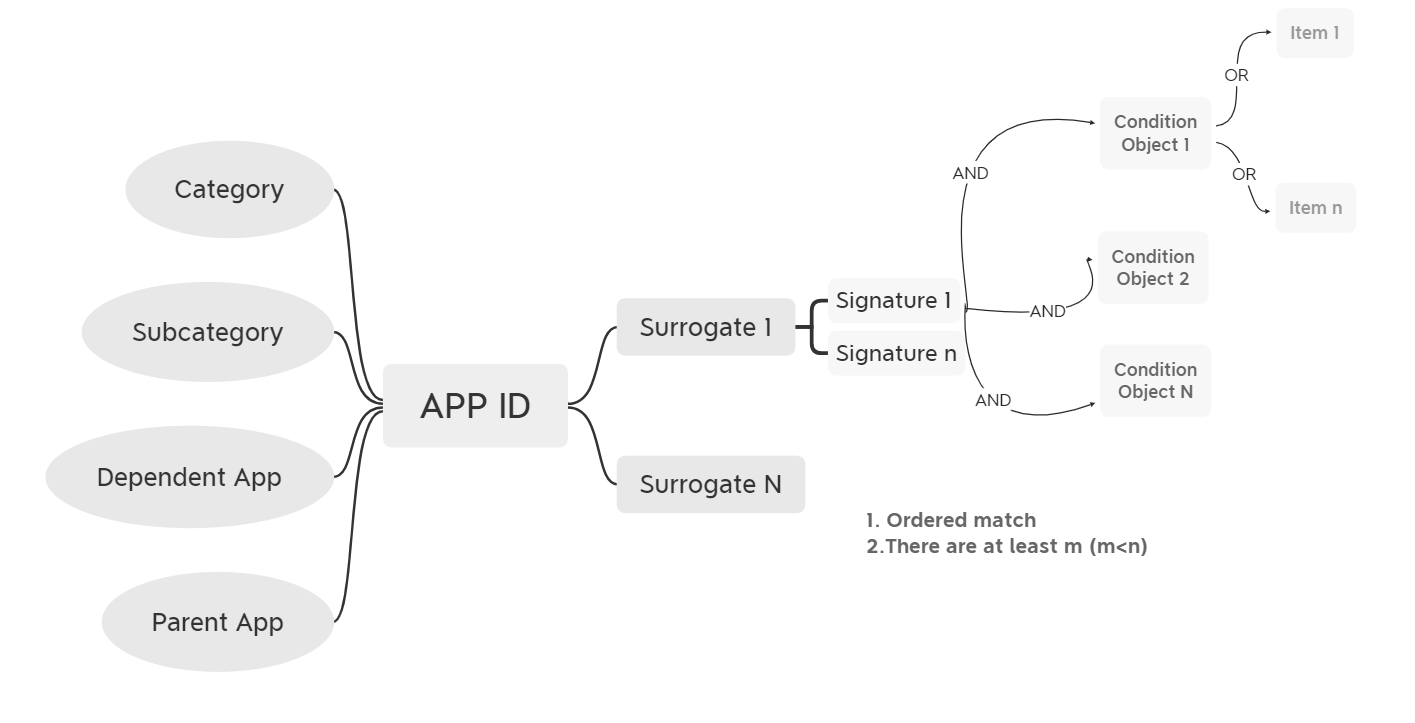
\includegraphics[width=\textwidth]{gfx/fig_signatures}
	%\caption{Figure: Inspection Stage}
	\label{fig:system:fig_signatures}
\end{figure}


The following demonstrates how to create a customized signature.

\begin{description}
    \item[STEP 1.]	Select \textbf{Objects} > \textbf{Applications}, select tab \textbf{Signatures} and click \textbf{Create}.
    \item[STEP 2.]	Add a \textbf{Name}. The name is case-sensitive and can have up to 128 characters.
    \item[STEP 3.]	Specify a \textbf{Color}.
    \item[STEP 4.]	(\textcolor{gold}{Optional})Enter a \textbf{Comment}.
    \item[STEP 5.]	Add \textbf{Conditions}. You can add one or multiple conditions. The relation between New Conditions is “and”, and the relation within existing condition is “or”. 
    Select \textbf{Attribute Name} and this affects the rest of the available selections. Fill in the corresponding content. Note that valid keywords length is from 4 to 1024 bytes.
    \item[STEP 6.]	Click \textbf{OK}.
\end{description}

\notemark\textit{Within the same signature, attributes from different protocols are not allowed to serve as Conditions, except for TCP/IP/General Attributes.}


You can \textbf{Edit} or \textbf{Delete} your signature and reference one or multiple signatures when creating application object.

\pdfbookmark[2]{Customized Attributes}{Customized Attributes}
\subsection*{\hypertarget{link:Customized Attributes}{Customized Attributes}}
\label{sec:objects:application:attribute}

The traffic attribute is the information obtained after the analysis of the network transmission unit. The attributes used by the App recognition can be found in \textbf{Appendix F Best Practice} > \textbf{\hyperlink{link:Custom Application}{\color{linkblue}{Custom Application}}}.


You can also upload a Lua script to create your own traffic attributes.


The following is a basic example of how to create a customized attribute.

\begin{description}
    \item[STEP 1.]	Select \textbf{Objects} > \textbf{Applications}, select tab \textbf{Customized Attributes} and click \textbf{Create}.
    \item[STEP 2.]	Add a \textbf{Name}. The name is case-sensitive and can have up to 128 characters.
    \item[STEP 3.]	Select \textbf{Parent Attribute} from traffic attribute list.
    \item[STEP 4.]	Please upload \textbf{Uploaded File}.
    \item[STEP 5.]	Select \textbf{Attribute Type} from: Bool, Numeric Value, and String.
    \item[STEP 6.]	Specify \textbf{Maximum Execution Time}.
    \item[STEP 7.]	Click \textbf{OK}.
\end{description}

\notemark\textit{Lua is a lightweight, high-level, multi-paradigm programming language designed primarily for embedded use in applications. TSG is able to interact with Lua scripts when process network traffic.}	


\notemark\textit{It is best practice to construct a Pre-Signature to improve performance when a customized attribute is referenced by Signature as a Condition.} 


You can \textbf{Edit} or \textbf{Delete} your customized attributes and download the Uploaded File.

\pdfbookmark[2]{Custom Application}{Custom Application}
\subsection*{\hypertarget{link:Custom Application}{Custom Application}}
\label{sec:objects:application:customize}

Applications allow you classify all traffic, across all ports, all the time. To ensure that your internal custom applications do not show up as unknown traffic, you can create a custom application. Then practice granular policy control over these applications to minimize the range of unidentified traffic on your network. 


To create a custom application, you must define the application attributes: its characteristics, category and sub-category, risk, port, timeout. In addition, you must define patterns or values that TSG can use to match to the traffic flows (the signature). Finally, you can attach the custom application to a policy that allows or denies the application (or add it to an application group or match it to an application selector).


\notemark\textit{In order to collect the right data to create a custom application signature, you'll need a good understanding of packet captures and how to analyze data pattern. If the signature is created too broadly, you might inadvertently include other similar traffic; if it is defined too narrowly, the traffic will evade detection if it does not strictly match the pattern.}


The following is a basic example of how to create a custom application.

\begin{description}
    \item[STEP 1.]	Gather information about the application to create custom signatures.


    To do this, you need have an understanding of the application and how you want to control access to it. For example, you may want to limit what operations users can perform within the application, such as uploading, downloading, or live streaming.


    • Capture application packets so that you can find unique characteristics about the application on which to base your custom application signature. One way to do this is to run a protocol analyzer, such as Wireshark, on the client system to capture the packets between the client and the server. Perform different actions in the application, such as uploading and downloading, so that you will be able to locate each type of session in the resulting packet captures (PCAPs).


    • Because TSG supports packet captures for all traffic, you can take packet captures using TSG. See \hyperlink{link:Take Packet Captures}{\color{linkblue}{Take Packet Captures}}.


    • Use the packet captures to find patterns or values in the packet contexts that you can use to create signatures that will uniquely match the application. For example, look for string patterns in HTTP request or response headers, URI, or hostnames.
    \item[STEP 2.]	Add the custom application.
    \begin{enumerate}  
        \item Select \textbf{Objects} > \textbf{Applications} and click \textbf{Create}.
        \item Enter a \textbf{Name} and a \textbf{Description} for the custom application that will help other administrators understand why you created the application.
        \item Verify that \textbf{Enabled} is enabled.
        

            Policy rules referencing applications only match to and enforce traffic based on enabled applications. 
        
        
            Predefined applications cannot be disabled and only allow a status of enabled. Disabling a base application could cause applications which depend on the base application to also be disabled. For example, disabling Facebook-base will disable all other Facebook applications.
        \item Define the application Properties and Characteristics.
        

            Select the \textbf{Category}, \textbf{Subcategory}, \textbf{Technology} and \textbf{Risk} from drop-down. Add \textbf{Parent App} if there is any. Enable \textbf{Continue Scanning} if you need to. Select the checkbox for characteristics, including Evasive, Excessive Bandwidth, Prone to Misuse, SaaS, Transfer Files, Tunnels Other Apps, Used by Malware, Vulnerability and Widely Used.
        \item Define the timeout values or leave the value set to default.
    \end{enumerate}
    \item[STEP 3.]	Define the Surrogates which is the criteria that the firewall will use to match the traffic to the new application.


        You will use the information you gathered from the packet captures to specify unique string context values that the firewall can use to match patterns in the application traffic.
             
        
        Select Signatures or click plus icon to create a signature.
    \begin{enumerate}
        \item On create a Signature page, define a Signature \textbf{Name} and optionally a \textbf{Comment} to provide information about how you intend to use this signature.
        \item Pick a \textbf{Color} or use the default color.
        \item Specify \textbf{Conditions} to define signatures.
        

            If the order in which the firewall attempts to match the signature definitions is important, make sure to enable the Ordered Match and then order the conditions so that they are evaluated in the appropriate order. Select a condition and click Move Up or Move Down.
    \end{enumerate}
    \item[STEP 4.]	Click \textbf{OK}.
    \item[STEP 5.]	Validate that traffic matches the custom application as expected.
    \begin{enumerate}
        \item Select \textbf{Policies} > \textbf{Security} and \textbf{Create} a security policy rule to allow the new application.
        \item Run the application from a client system that is between the firewall and the application and then check the logs to make sure that you see traffic matching the new application (and that it is being handled per your policy rule).
    \end{enumerate}
\end{description}

\pdfbookmark[2]{Application Selector}{Application Selector}
\subsection*{\hypertarget{link:Application Selector}{Application Selector}}
\label{sec:objects:application:selector}

An application selector is an object that dynamically groups applications based on application attributes that you define, including category, subcategory, technology, risk and characteristics. This is useful when you want to enable access to applications that you do not explicitly sanction, but that you want users to be able to access. For example, you may want to enable employees to choose their own office programs, such as Evernote, Google Docs, or Microsoft Office, for business use. To enable these types of applications, you could create an application selector that matches on the Category business-systems and the Subcategory office-programs. As new applications office programs emerge, these new applications will automatically match the selector you defined; you don’t have to make any additional changes to your policy rules to enable any application that matches the attributes you defined for the selector.

\begin{description}
    \item[STEP 1.]	Select \textbf{Objects} > \textbf{Applications} > \textbf{Selectors}.
    \item[STEP 2.]	Create a selector and give it a descriptive \textbf{Name}.
    \item[STEP 3.]	Define the selector by selecting attribute values from the Category, Subcategory, Technology, Risk, and Characteristics sections. 
    As you select values, notice that the list of matching applications at the bottom of the dialog narrows. 
    When you have adjusted the filter attributes to match the types of applications you want to safely enable, click \textbf{OK}.
\end{description}

\pdfbookmark[2]{Application Group}{Application Group}
\subsection*{\hypertarget{link:Application Group}{Application Group}}
\label{sec:objects:application:group}

An application group is an object that contains applications that you want to treat similarly in a policy. Application groups are useful for allow or deny access to applications that you explicitly sanction or forbid. Grouping sanctioned or forbidden applications simplifies administration of your rules. Instead of having to update individual policy rules when there is a change in the applications you sanction or deny, you can update only the affected application groups.


When deciding how to group applications, consider how you plan to enforce access to your applications and create an application group that aligns with each of your policy goals. For example, you might have some applications that you will allow, and other applications that you want to deny. In this case, you would create separate application groups for each of these policy goals.

\begin{description}
    \item[STEP 1.]	Select \textbf{Objects} > \textbf{Applications} > \textbf{Groups}.
    \item[STEP 2.]	Create a group and give it a descriptive \textbf{Name}.
    \item[STEP 3.]	Add the applications you want in the group.
    \item[STEP 4.]	(\textcolor{gold}{Optional}) Enter a \textbf{Description} or leave the value set to empty. Description can have up to 1024 characters.
    \item[STEP 5.]	Click \textbf{OK}.    
\end{description}

\pdfbookmark[1]{Configure Object Group}{Configure Object Group}
\section*{\hypertarget{link:Configure Object Group}{Configure Object Group}}
\label{sec:objects:group}

A policy object consists of one or multiple items, while an object group is composed of one or multiple subordinate objects. An object group is also considered as an object. Typically, when creating a policy object, you organize objects that require similar permissions in policy. One object is allowed to reference same type objects as subordinate objects, but not allowed to add items in object. For example, An IP object defines a set of single address, whereas an IP object group can define more than one address object. By grouping objects, you can significantly reduce the administrative overhead in creating policies. You can create object group for all types of objects.


The following procedure explains how you can create objects group directly through the Objects page.

\begin{description}
    \item[STEP 1.]	Select \textbf{Objects}, then select the menu you want to create from the following: IP addresses, FQDNs, Subscriber IDs, HTTP Signatures, Keywords, URLs, Categories, Accounts.
    \item[STEP 2.]	To create a group, let’s take FQDN as an example, click \textbf{Create} and select FQDN group.
    \item[STEP 3.]	Add a \textbf{Name}. The name is case-sensitive and can have up to 128 characters.
    \item[STEP 4.]	Specify a \textbf{Color}.
    \item[STEP 5.]	Add one or more \textbf{Sub Objects}. Note that you cannot add sub objects and items at the same time.
    \item[STEP 6.]	(\textcolor{gold}{Optional})Enter a \textbf{Description}. The description can have up to 1024 characters.
    \item[STEP 7.]	Click \textbf{OK}.    
\end{description}